%%%%%%%%%%%%%%%%%%%%%%%%%%%%%%%%%%%%%%%%%
% Journal Article
% LaTeX Template
% Version 1.3 (9/9/13)
%
% This template has been downloaded from:
% http://www.LaTeXTemplates.com
%
% Original author:
% Frits Wenneker (http://www.howtotex.com)
%
% License:
% CC BY-NC-SA 3.0 (http://creativecommons.org/licenses/by-nc-sa/3.0/)
%
%%%%%%%%%%%%%%%%%%%%%%%%%%%%%%%%%%%%%%%%%

%----------------------------------------------------------------------------------------
%	PACKAGES AND OTHER DOCUMENT CONFIGURATIONS
%----------------------------------------------------------------------------------------

\documentclass[twoside]{article}
\usepackage{graphicx}

\usepackage[sc]{mathpazo} % Use the Palatino font
\usepackage[T1]{fontenc} % Use 8-bit encoding that has 256 glyphs
\linespread{1.05} % Line spacing - Palatino needs more space between lines
\usepackage{microtype} % Slightly tweak font spacing for aesthetics

\usepackage[hmarginratio=1:1,top=32mm,columnsep=20pt]{geometry} % Document margins
\usepackage{multicol} % Used for the two-column layout of the document
\usepackage[hang, small,labelfont=bf,up,textfont=it,up]{caption} % Custom captions under/above floats in tables or figures
\usepackage{booktabs} % Horizontal rules in tables
\usepackage{float} % Required for tables and figures in the multi-column environment - they need to be placed in specific locations with the [H] (e.g. \begin{table}[H])
\usepackage{hyperref} % For hyperlinks in the PDF

\usepackage{lettrine} % The lettrine is the first enlarged letter at the beginning of the text
\usepackage{paralist} % Used for the compactitem environment which makes bullet points with less space between them

\usepackage{abstract} % Allows abstract customization
\renewcommand{\abstractnamefont}{\normalfont\bfseries} % Set the "Abstract" text to bold
\renewcommand{\abstracttextfont}{\normalfont\small\itshape} % Set the abstract itself to small italic text

\usepackage{titlesec} % Allows customization of titles
\renewcommand\thesection{\Roman{section}} % Roman numerals for the sections
\renewcommand\thesubsection{\arabic{subsection}} % Roman numerals for subsections
\titleformat{\section}[block]{\large\scshape\centering}{\thesection.}{1em}{} % Change the look of the section titles
\titleformat{\subsection}[block]{\large}{\thesubsection.}{1em}{} % Change the look of the section titles

\usepackage{fancyhdr} % Headers and footers
\pagestyle{fancy} % All pages have headers and footers
\fancyhead{} % Blank out the default header
\fancyfoot{} % Blank out the default footer
\fancyhead[C]{PPGEB - FEELT - UFU $\bullet$ 2013/2} % Custom header text
\fancyfoot[RO,LE]{\thepage} % Custom footer text

\usepackage[brazilian]{babel}
\usepackage[utf8]{inputenc}
\usepackage[T1]{fontenc}
\usepackage{graphicx}
\graphicspath{{imgs/}}

\usepackage{listings}
\usepackage{xcolor}

\lstdefinestyle{sharpc}{language=[Sharp]C, frame=lr, rulecolor=\color{blue!80!black}, breaklines=true}

%----------------------------------------------------------------------------------------
%	TITLE SECTION
%----------------------------------------------------------------------------------------

\title{\vspace{-15mm}\fontsize{24pt}{10pt}\selectfont\textbf{Desenvolvimento de um recurso de previsão de texto para um software de CAA, destinado para pacientes com limitação motora severa.}} % Article title

\author{
\large
\textsc{CURTT J.R., FERREIRA L.C.V., LIMA M.A.B., MARIANO D.T.G., NAVES E.L.M.}\\[2mm] % Your name
\normalsize \\Laboratório de Engenharia Biomédica \\Faculdade de Engenharia Elétrica \\Núcleo de Tecnologias Assistivas \\Universidade Federal de Uberlândia\\ \normalsize Uberlândia-MG, Brasil \\ % Your institution
\normalsize {jrcurttjr@msn.com, lcv.ferreira@yahoo.com.br, borba.lima@hotmail.com, dtgmariano@gmail.com}
\vspace{-5mm}
}
\date{}

%----------------------------------------------------------------------------------------

\begin{document}
\maketitle % Insert title
\thispagestyle{fancy} % All pages have headers and footers

%----------------------------------------------------------------------------------------
%	ABSTRACT
%----------------------------------------------------------------------------------------


\begin{abstract}
\noindent
Predição de texto é uma das técnicas mais utilizadas para melhorar a taxa de comunicação em comunicação aumentativa e alternativa. Sistemas de previsão são tradicionalmente usados por pessoas com deficiência (por exemplo, as pessoas com deficiencias motoras e de fala). Este artigo apresenta o desenvolvimento de uma ferramenta de previsão de texto para um software de comunicação alternativa e aumentada, voltado para pacientes portadores de disfunções motoras graves.
\end{abstract}

%----------------------------------------------------------------------------------------
%        ARTICLE CONTENTS
%----------------------------------------------------------------------------------------

\begin{multicols}{2} % Two-column layout throughout the main article text

\section{Introdução}
\subsection{Tecnologias assistivas}
Uma das principais formas de socialização que o ser humano possui é a fala, que lhe garante o entendimento por outros, de seus anseios e desejos. No Brasil, conforme o censo realizado em 2010 pelo IBGE existe cerca de 45,6 milhões de pessoas com deficiência, o que representa 23,9\% da população brasileira, sendo que grande parte destas pessoas possui um ou mais tipos de deficiência, podendo ser física, visual, auditiva, intelectual ou de comunicação [1].
\\\\
Ao analisar a vida cotidiana do ser humano, é possível dizer que uma gama de fatores podem influenciar suas atitudes e atividades diárias, seja no trabalho ou na vida social, para isto se faz necessário englobar uma análise ergonômica de suas atividades, para saber como estas situações, seja de forma positiva ou negativa, afetam o indivíduo nas questões físicas, sociais ou psicológicas.  A palavra Ergonomia é de origem grega sendo, ergo significando tarefa, por extensão trabalho, e nomos normas, regras [2].
\\\\
Assim sendo ergonomia pode ser definida como uma abordagem científica que se fundamenta em conhecimentos interdisciplinares das ciências humanas para, de um lado, compatibilizar os produtos e as tecnologias com as características dos usuários e, de outro, humanizar o contexto sociotécnico de trabalho, adaptando-o tanto aos objetivos do sujeito e/ou grupo, quanto às exigências das tarefas [3;4]. 
\\\\
Com o estudo da ergonomia surge uma área de grande importância para a adaptação do deficiente à vida em sociedade, que é a tecnologia assistiva (TA), que é utilizado para identificar todo o arsenal de recursos e serviços que contribuem para proporcionar ou ampliar habilidades funcionais de pessoas com deficiência e consequentemente promover vida independente e inclusão. Podendo ser definido ainda como, uma ampla gama de equipamentos, serviços, estratégias e práticas concebidas e aplicadas para minorar os problemas funcionais encontrados pelos indivíduos com deficiências [5].
\\\\
Faz-se necessário realizar ou promover a pesquisa e o desenvolvimento, bem como a disponibilidade e o emprego de novas tecnologias, inclusive as tecnologias da informação e comunicação, ajudas técnicas para locomoção, dispositivos e tecnologias assistivas, adequados a pessoas com deficiência, dando prioridade a tecnologias de custo acessível [6].
\\\
Por assim ser, há a necessidade de se desenvolver instrumentos que facilitem à socialização destas pessoas com deficiência, seja através da forma mais simples ou da forma mais complexa (cartilhas de comunicação, ambientes adaptados, softwares, hardwares, etc.) estes instrumentos são conhecidos como tecnologia assistiva [7].
\\\\
Desta forma, tecnologia assistiva é qualquer produto, instrumento, equipamento ou sistema técnico utilizado por uma pessoa incapacitada, que se destina a prevenir, compensar, monitorizar, aliviar ou neutralizar a incapacidade [8].
\\\\
Os recursos e serviços de tecnologia assistiva são organizados ou classificados de acordo com objetivos funcionais a que se destinam, tais como mobilidade, adequação postural, comunicação, recursos para cegos ou pessoas de baixa visão, para surdos ou pessoas com perdas auditivas, instrumentos que promovam independência em atividades da vida diária, recursos para educação, recreação, acessibilidade arquitetônica, adaptações de veículos, recursos para acesso ao computador, órteses, próteses e outros [9].
\\\\
Recursos de comunicação podem ser dos mais variados tipos. Projeta-se e constrói-se um recurso considerando as habilidades do usuário com o objetivo de ajudá-lo a superar sua deficiência. Um recurso após ser desenvolvido e aplicado poderá ser então aperfeiçoado, considerando as dificuldades de adaptação do indivíduo [9]. 
\\\\
Para atender pessoas sem fala, sem escrita funcional ou em defasagem entre sua necessidade comunicativa e sua habilidade em falar e/ou escrever, são utilizados recursos conhecidos como comunicação aumentativa e alternativa (CAA). A CAA serve para expressar suas questões, desejos, sentimentos, entendimentos. A alta tecnologia dos vocalizadores (pranchas com produção de voz) ou o computador com softwares específicos garantem grande eficiência à função comunicativa [5].

\subsection{Disfunções motoras severas}
Distúrbios neurológicos como a esclerose lateral amiotrófica (ELA) ou outras doenças musculares progressivas, conduzem frequentemente esses indivíduos à paralisia motora, inclusive com prejuízo a fala. Tornam-se, portanto, altamente limitados para suas atividades, inclusive com privação de suas vontades, devido à perda de comunicação.
\\\\
Esta patologia atinge cerca de 1 a 3 novos casos por cada 100,000 habitantes anualmente, tendo uma prevalência detida entre os 3 e os 7 por 100,000 habitantes/ano. Ainda por razões desconhecidas, o sexo masculino tem um predominância ligeiramente superior quando comparado com o feminino, com uma proporção M:F de 1,5:1 [10]. 
\\\\
Habitualmente a idade média de aparecimento da doença ocorre entre os 55-65 anos de idade, embora em  alguns casos, cerca de 5\% possa manifestar-se a partir da segunda década de vida [11].
\\\\
Para alguns desses indivíduos o sistema de escaneamento é o único modo de acesso à comunicação verbal ou escrita. Esses fundamentos têm sido utilizados desde o início da década de 80: através de um sistema de varredura luminosa, um item é marcado na tela e então selecionado por um clique.
\\\\
A principal desvantagem desse método é a lentidão na comunicação com uma velocidade média de escaneamento entre 0,2 a 6 segundos [7].

\subsection{EDITH}
O EDITH (acronismo francês para Ambiente de Teleação Digital para Pessoas com Disfunções), desenvolvido na Universidade Metz, França, é um software de CAA, desenvolvido para pessoas com Esclerose Lateral Amiotrofica.

\begin{figure}[H]
\label{fig:edith_menu}
  \caption{Menu do EDITH.}
  \centering
    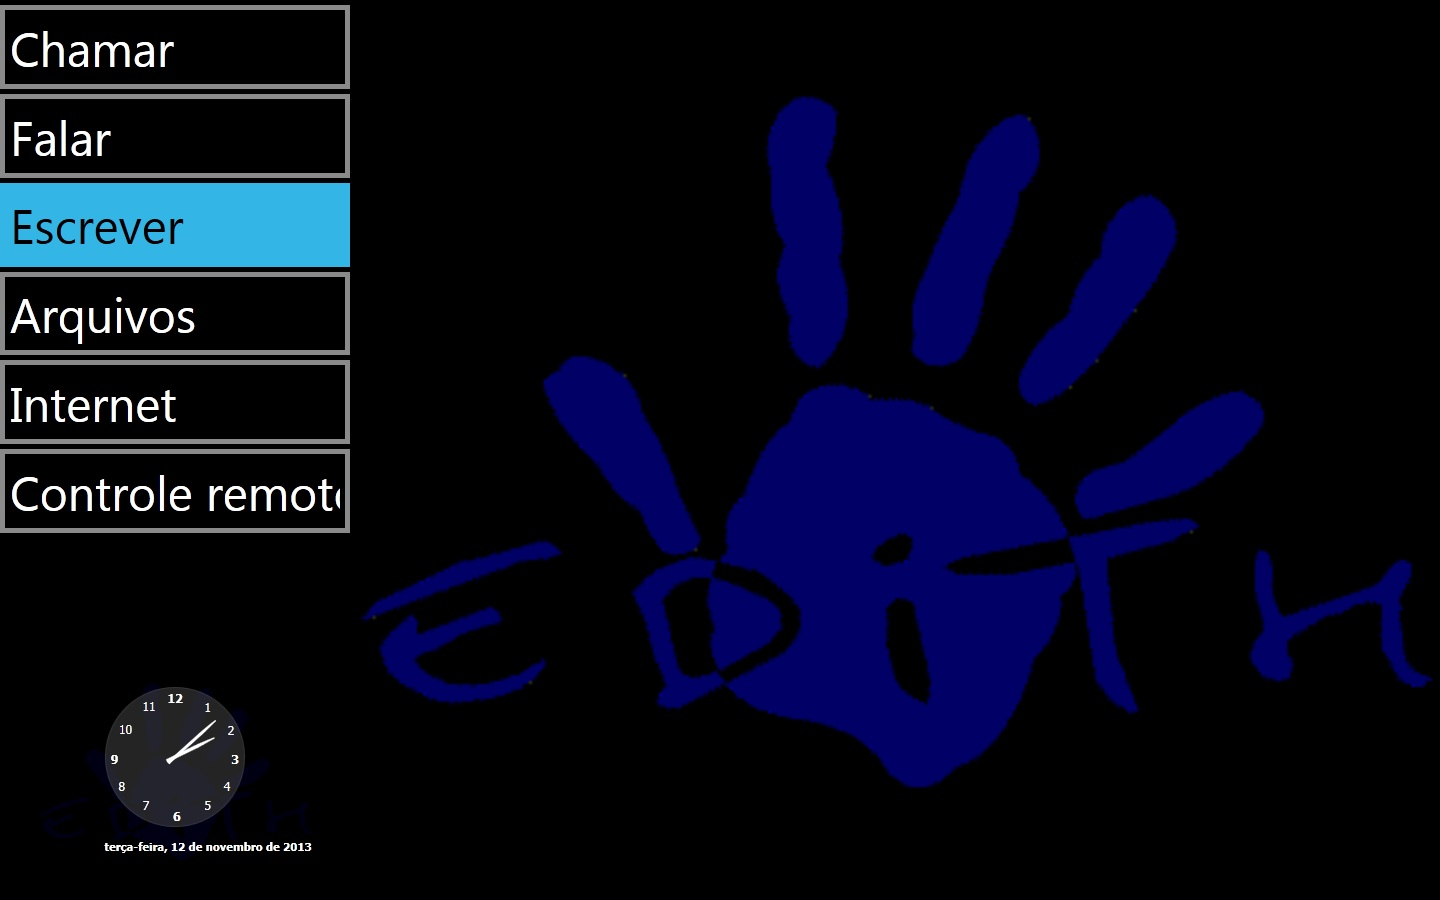
\includegraphics[scale = 0.19]{edith_menu.png}
\end{figure}

\noindent Trata-se de um sistema de auxílio à comunicação destinada a pessoas com deficiências motoras severas e que não estão aptas a se comunicarem. Ele é composto por um software que integra diversos recursos para controle de um ambiente multimídia de comunicação. 
\noindent \\\\Para o sistema de seleção costuma-se aplicar o modo linha-coluna (ou coluna-linha), por proporcionar um menor dispêndio de esforço físico e mental nessas ações. O sistema de seleção pode também ser sequencial, se a disponibilidade de opções não for muito ampla. 

\begin{figure}[H]
\label{fig:edith_tecladovirtual}
  \caption{Teclado virtual.}
  \centering
    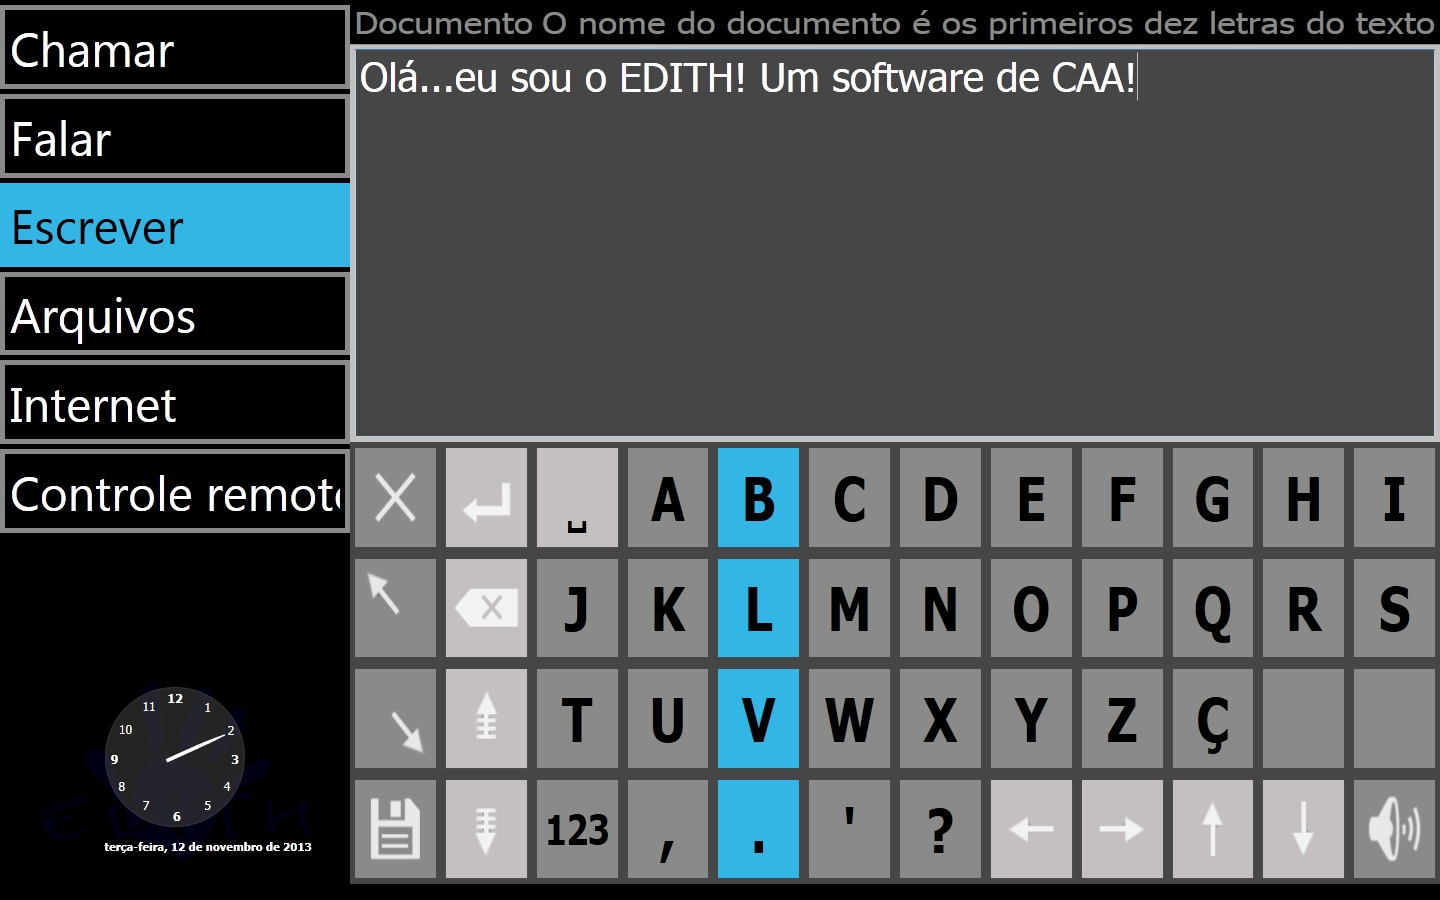
\includegraphics[scale = 0.19]{edith_tecladovirtual.png}
\end{figure}

\noindent É possível ajustar o parâmetro temporal de acordo com a personalidade e as habilidades físicas e cognitivas do usuário; pode ser diminuído quando o usuário adquirir experiência com a interface, ou aumentado, se houver deterioração da função por agravo da enfermidade. 

\noindent \\O sistema EDITH foi projetado para computadores padrão IBM-PC e possui duas componentes principais: uma interface funcional e uma interface de configuração. A interface funcional oferece várias facilidades como avisos e chamadas sonoras do pessoal de enfermagem, leitura de textos e escrita de texto. A interface de configuração permite ao usuário ajustar a operação de diversas funcionalidades como tempo de varredura do teclado virtual, adicionar livros, filmes, músicas no banco de dados e cadastrar e-mails.

\begin{figure}[H]
\label{fig:edith_chamar}
  \caption{Módulo para chamada urgente.}
  \centering
    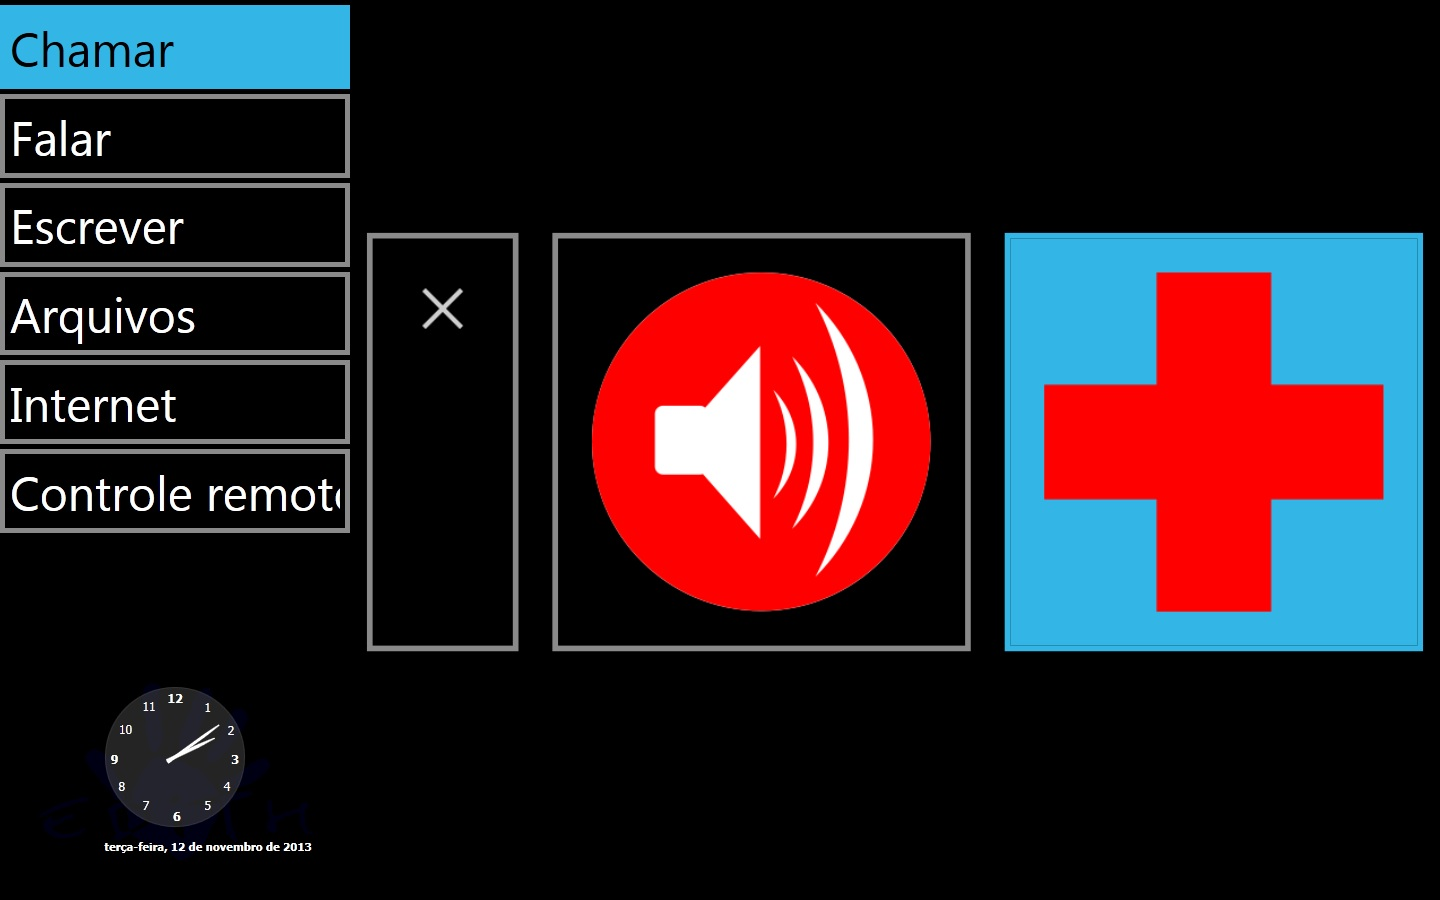
\includegraphics[scale = 0.19]{edith_chamar.png}
\end{figure}

\noindent O software foi desenvolvido na plataforma de desenvolvimento .NET da Microsoft, utilizando linguagem computacional C\# (CSharp). O aplicativo possui um gerador de registros (log) que grava as ações desempenhadas pelo usuário durante a execução do programa. O objetivo de vários pesquisadores que atuam na área de tecnologia assistiva tem sido a de aperfeiçoar esses softwares para uma melhor adaptação do usuário com a interface, permitindo menor esforço físico e melhor aproveitamento desses recursos. Indivíduos com disfunções motoras associados a distúrbios da fala frequentemente utilizam-se de recursos de comunicação como o EDITH, contudo, devido a velocidade que a escrita é executada, às vezes por limitações físicas desses pacientes, esses dispositivos tornam essa capacidade de comunicação uma tarefa de difícil execução. 

%------------------------------------------------
\section{Métodos}

\subsection{Experimento}
Esta é uma pesquisa do tipo experimental quantitativa, baseada em dados estatísticos. Com o objetivo de melhorar a velocidade de comunicação e diminuir esforços aos usuários do software EDITH, foi desenvolvido uma ferramenta “autocompletar” ao teclado virtual, com o intuito de exigir um menor número de cliques para digitar uma palavra. Para isto serão realizados alguns testes comparando a performance de usuários utilizando o recurso autocompletar e sem o mesmo. Os voluntários foram classificados como indivíduos saudáveis, não sendo portadores de nenhuma disfunção motora. 
\\\\
Para estipular a sentença a ser usada para o teste, optou-se pelo emprego de um pangrama. Um pangrama é uma frase com sentido em que são usadas todas as letras do alfabeto de determinada língua. O pangrama utilizado para o teste possui 42 letras, sendo expresso pela seguinte frase: "Um pequeno jabuti xereta viu dez cegonhas felizes". 
\\\\
Com base nos registros de eventos (log) do software, serão analisados os seguintes parâmetros oriundos da atividade de escrita com o software:
\begin{itemize}
\item Número de cliques executados pelo usuário;
\item Intervalo médio entre os cliques;
\item Taxa de acerto (\%);
\item Taxa de erro(\%);
\end{itemize}

\subsection{Tratamento dos registros}

O EDITH registra todos os eventos de clique do usuário, armazenando a data, hora, tipo de ação e seu detalhe. A seguir pode-se visualizar um exemplo de log gerado pelo programa.

\begin{lstlisting}
2013-12-20 18:34:19,817 
ActionKeySelectedFirstKeyboard|
Key : U
\end{lstlisting}

Com base em sua estrutura, cada evento foi classificado nos seguintes tipos de ação:
\begin{itemize}

\item Key Selected FirstKeyboard
\hfill \\
  "Key" significa que algum caractere foi pressionado.
\item Backspace Selected FirstKeyboard
\hfill \\
  "Backspace" significa que a tecla de retroceder foi pressionada.
\item Column Selected FirstKeyboard
\hfill \\
  "Column" significa que a alguma coluna do teclado virtual foi selecionada durante a sua varredura.
\item Space Selected FirstKeyboard
\hfill \\
  "Space" significa que foi inserido um espaço vazio na caixa de texto.
\item Speech Selected FirstKeyboard
\hfill \\
  "Speech" significa que o botão para reproduzir em áudio a frase armazenada na caixa de texto.
\end{itemize}

\noindent Foram definidos como cliques do usuário todos os eventos disparados ("Key", "Backspace", "Column", "Space", "Speech", entre outros). A taxa de acerto foi definido como o total de caracteres digitados (associado aos eventos "Key" e "Space") subtraídos do número de caracteres que foram digitados de maneira errada. A taxa de erro, composta pelo número de caracteres digitados erroneamente, está associado ao disparo do evento "Backspace".
A sensibilidade das letras serem maiúsculas ou minúsculas foi ignorada para esta aplicação, uma vez que este fator não atrapalhar o desempenho da comunicação.

%------------------------------------------------
\section{Resultados}

Após os ensaios foram coletados os seguintes dados dos usuários e organizados nas seguintes tabelas:

\begin{table}[H]
\caption{Dados do usuário 1}
\centering
\begin{tabular}{ccc}
\toprule
 Usuário 1 &  & \\
\midrule
Autocompletar & Não & Sim\\
Duração (ms) & 282394 & 508249\\
Número de cliques & 118 & 147\\
Tempo médio por clique & 2393.17 & 3457.48\\
N. de caracteres & 51 & 49\\
N. de caracteres errados & 3 & 17\\
Acerto (\%) & 94.12 & 65.31\\
Erro (\%) & 5.88 &\ 34.69\\
\bottomrule
\end{tabular}
\end{table}


\begin{table}[H]
\caption{Dados do usuário 2}
\centering
\begin{tabular}{ccc}
\toprule
 Usuário 2 &  & \\
\midrule
Autocompletar & Não & Sim\\
Duração (ms) & 243062 & 383033\\
Número de cliques & 116 & 136\\
Tempo médio por clique & 2095.36 & 2816.42\\
N. de caracteres & 51 & 46\\
N. de caracteres errados & 2 & 18\\
Acerto (\%) & 96.08 & 60.87\\
Erro (\%) & 3.92 &\ 39.13\\
\bottomrule
\end{tabular}
\end{table}

\noindent Com base dos dados foram construídos os seguintes gráficos para comparação entre as parâmetros estatísticos dos experimentos sem o uso da ferramenta de autocomplemento e com o seu uso:

\begin{figure}[H]
\label{fig:graph_tx}
  \caption{Taxa percentual de acerto e erro}
  \centering
    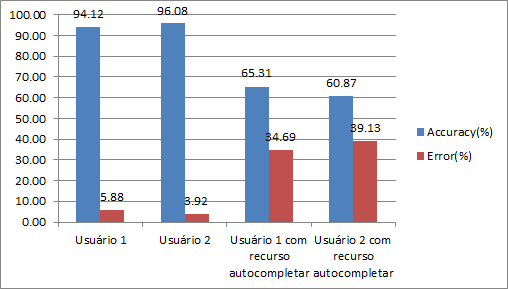
\includegraphics[scale = 0.50]{graph_acertoerro.png}
\end{figure}

\begin{figure}[H]
\label{fig:graph_d}
  \caption{Duração da tarefa (em s)}
  \centering
    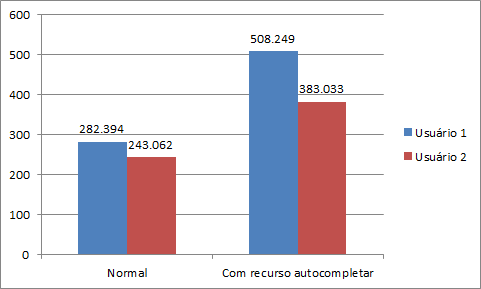
\includegraphics[scale = 0.50]{graph_duracao.png}
\end{figure}

\begin{figure}[H]
\label{fig:graph_int}
  \caption{Intervalo médio entre cliques (em ms)}
  \centering
    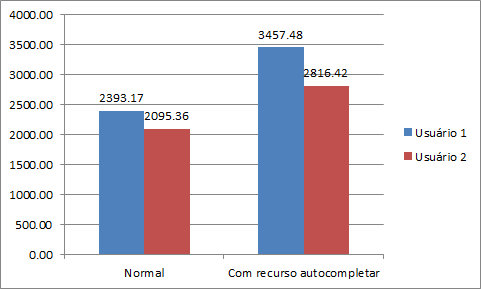
\includegraphics[scale = 0.50]{graph_intervalomed.png}
\end{figure}

\begin{figure}[H]
\label{fig:graph_numcliq}
  \caption{Número de cliques efetuados durante a tarefa}
  \centering
    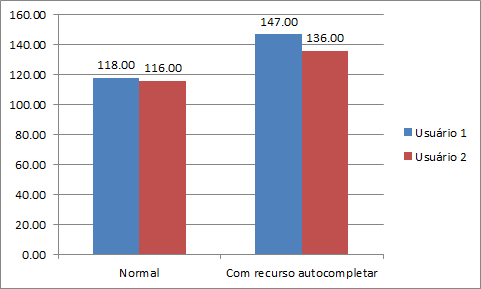
\includegraphics[scale = 0.50]{graph_ncliques.png}
\end{figure}

\begin{figure}[H]
\label{fig:graph_numcaractnec}
  \caption{Número caracteres necessários para completar a tarefa}
  \centering
    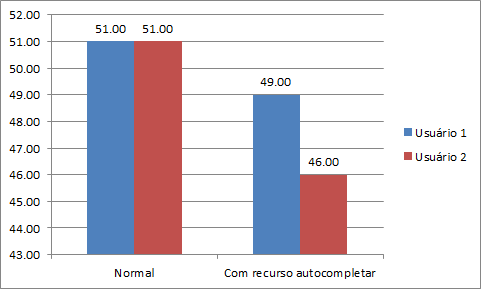
\includegraphics[scale = 0.50]{graph_caractnec.png}
\end{figure}

%-----------------------------------------------
\section{Discussão}
Os resultados apontaram que o recurso de autocomplemento, na atual configuração, ainda não está adequado para uso. O aumento de tempo de 39\% e do número de cliques de 21\% para escrever a sentença podem ser interpretadas como ineficiência da atual ferramenta. Entretanto, tal problema pode ser justificado pelo fato de o recurso de autocomplemento selecionar palavras independente da relevância sintática que esta possui dentro da frase. 

\noindent \\A dificuldade de se encontrar dicionários da lingua portuguesa, com valores de relevância pré-determinados, obrigou o desenvolvimento de um banco de dados com palavras sem atribuição deste atributo. Dessa forma, a busca por palavras no banco de dados se restringe a palavras iniciadas pelos caracteres digitados pelo usuário. 

\noindent \\Para um caso em que o usuário digite os caracteres 'A' e 'B', serão retornadas algumas palavras pertencente ao espaço amostral de palavras do dicionário, iniciadas por "AB", independente da frequência com que a palavra é utilizada ou de seu contexto sintático. Isso acarreta no incremento da probabilidade do recurso autocompletar sugerir palavras que não atendam à necessidade do usuário, uma vez que a ferramenta limita o número de palavras sugeridas, afim de evitar um grande consumo de tempo durante a varredura por estas.

\noindent \\O recurso instalado nesta aplicação é uma ferramenta estática, uma vez que não utiliza estratégias computacionais que possibilitem a aprendizagem do sistema, de forma a ajustar o atributo "peso" das palavras do dicionário.

\noindent \\Em detrimento do aumento da quantidade de cliques efetuados pelo usuário, o número de caracteres necessários para gerar a sentença foi reduzido para um valor em torno de 7\%. Tal fator aponta o potencial da ferramenta que necessita de estratégias mais adequadas para atenuar os problemas detectados nos resultados do experimento.

\noindent \\Após o experimento a busca por estratégias de análise de contexto, dicionários compostos por palavras com pesos associados a sua relevância sintática ou frequência de uso, são as possibilidades mais viáveis para que a melhoria do uso do sistema tenha êxito.

%----------------------------------------------------------------------------------------
%        REFERENCE LIST
%----------------------------------------------------------------------------------------

\begin{thebibliography}{99} % Bibliography - this is intentionally simple in this template

\bibitem _CEPES/IEUFU. Levantamento de Informações econômico-sociais da População Portadora de Deficiência no Município de Uberlândia-MG. UFU 2005.

\bibitem _CUNHA, A. G. Dicionário etimológico Nova Fronteira da língua portuguesa. FRONTEIRA, N. Rio de Janeiro 1982.

\bibitem _DANIELLOU, F., Ed. L’ergonomie en quête de ses principes. Débats épistémologiques. Toulouse, França: Octares Editionsed. 1996.

\bibitem _MONTMOLLIN, M., Ed. L'ergonomie. Paris, Editions La Découverte ed. 1990.

\bibitem _COOK, A. M. H., S. M. Assistive Technologies: Principles and Practices. Mosby. YEAR BOOK, I. St. Louis, Missouri 1995.

\bibitem _BRASIL. Experiências Educacionais Inclusivas. Programa Educação Inclusiva Direito à Diversidade. ESPECIAL., M. D. E. S. D. E. Brasília 2007.

\bibitem _ROCHA, L. A. D. A. D. INTERFACE MULTIMODAL APLICADA À COMUNICAÇÃO ALTERNATIVA PARA PESSOAS COM DEFICIÊNCIAS MOTORAS GRAVES. 2013.   Departamento de Engenharia Elétrica, Universidade Federal de Uberlândia, Uberlândia.

\bibitem _BRASIL. Decreto 5.296 de 02 de dezembro de 2004. FEDERAL, G. Brasília. Decreto 5.296 2004.

\bibitem _BERSCH, R. M. H., PASSERINO, L. M., BATISTA, V. J. Tecnologia Assistiva e Design na Realidade Brasileira. Anais do Terceiro Workshop Design e Materiais da UFRGS. Porto Alegre, RS 2007.

\bibitem _TURNER MR, H. O., BENATAR M, BROOKS BR, CHIO A, DE CARVALHO M, ET AL. Controversies and priorities in amyotrophic lateral sclerosis. Lancet Neurologyogy, v. 12, p. 310-322,  2013.   

\bibitem _HAUSER SL, F., AS, EUGENE B, KASPER DL, LONGO DL, JAMESON JL, LOSCALZO J. Amyotrophic Lateral Sclerosis and Other Motor Neuron Diseases. Estados Unidos da América: McGraw-Hill Companies: 358-363 p. 2010.

\end{thebibliography}

%----------------------------------------------------------------------------------------

\end{multicols}
\end{document}